


\tikzset{every picture/.style={line width=0.75pt}} %set default line width to 0.75pt        

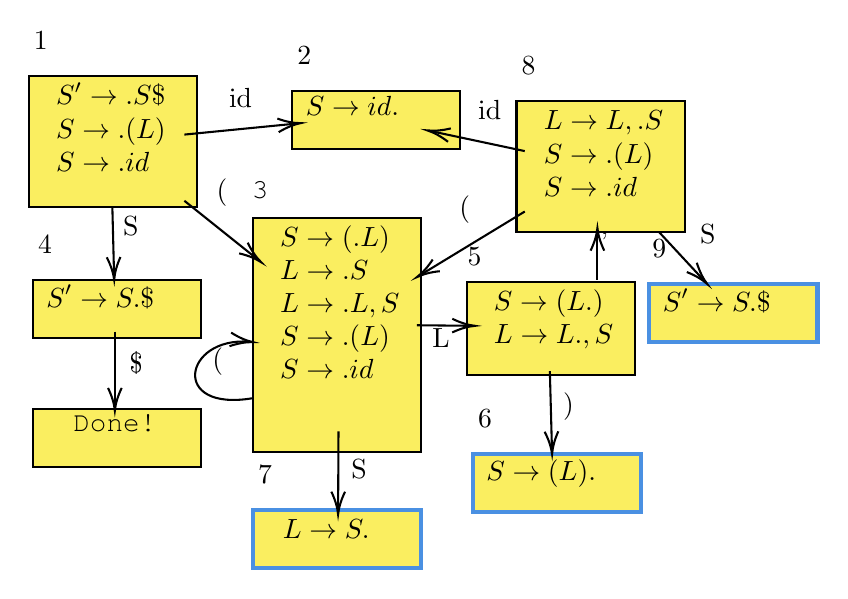
\begin{tikzpicture}[x=0.75pt,y=0.75pt,yscale=-1,xscale=1]
%uncomment if require: \path (0,719); %set diagram left start at 0, and has height of 719

%Shape: Rectangle [id:dp5944428075861247] 
\draw  [fill={rgb, 255:red, 248; green, 231; blue, 28 }  ,fill opacity=0.7 ] (21,36) -- (102,36) -- (102,99) -- (21,99) -- cycle ;
%Shape: Rectangle [id:dp6175437952862304] 
\draw  [fill={rgb, 255:red, 248; green, 231; blue, 28 }  ,fill opacity=0.7 ] (148,43) -- (229,43) -- (229,71) -- (148,71) -- cycle ;
%Shape: Rectangle [id:dp9636988265906923] 
\draw  [fill={rgb, 255:red, 248; green, 231; blue, 28 }  ,fill opacity=0.7 ] (23,134) -- (104,134) -- (104,162) -- (23,162) -- cycle ;
%Shape: Rectangle [id:dp514688489136807] 
\draw  [fill={rgb, 255:red, 248; green, 231; blue, 28 }  ,fill opacity=0.7 ] (23,196) -- (104,196) -- (104,224) -- (23,224) -- cycle ;
%Shape: Rectangle [id:dp4559883564568191] 
\draw  [fill={rgb, 255:red, 248; green, 231; blue, 28 }  ,fill opacity=0.7 ] (129,104) -- (210,104) -- (210,217) -- (129,217) -- cycle ;
%Shape: Rectangle [id:dp2829754007322226] 
\draw  [fill={rgb, 255:red, 248; green, 231; blue, 28 }  ,fill opacity=0.7 ] (256,48) -- (337,48) -- (337,111) -- (256,111) -- cycle ;
%Shape: Rectangle [id:dp10146079037621025] 
\draw  [color={rgb, 255:red, 74; green, 144; blue, 226 }  ,draw opacity=1 ][fill={rgb, 255:red, 248; green, 231; blue, 28 }  ,fill opacity=0.7 ][line width=1.5]  (320,136) -- (401,136) -- (401,164) -- (320,164) -- cycle ;
%Shape: Rectangle [id:dp1615821200335068] 
\draw  [fill={rgb, 255:red, 248; green, 231; blue, 28 }  ,fill opacity=0.7 ] (232,135) -- (313,135) -- (313,180) -- (232,180) -- cycle ;
%Shape: Rectangle [id:dp6257738628786156] 
\draw  [color={rgb, 255:red, 74; green, 144; blue, 226 }  ,draw opacity=1 ][fill={rgb, 255:red, 248; green, 231; blue, 28 }  ,fill opacity=0.7 ][line width=1.5]  (235,218) -- (316,218) -- (316,246) -- (235,246) -- cycle ;
%Shape: Rectangle [id:dp4964608877579646] 
\draw  [color={rgb, 255:red, 74; green, 144; blue, 226 }  ,draw opacity=1 ][fill={rgb, 255:red, 248; green, 231; blue, 28 }  ,fill opacity=0.7 ][line width=1.5]  (129,245) -- (210,245) -- (210,273) -- (129,273) -- cycle ;
%Curve Lines [id:da39507608620567136] 
\draw    (129,191) .. controls (88.82,197.86) and (95.7,161.5) .. (127.05,163.81) ;
\draw [shift={(129,164)}, rotate = 186.91] [color={rgb, 255:red, 0; green, 0; blue, 0 }  ][line width=0.75]    (10.93,-3.29) .. controls (6.95,-1.4) and (3.31,-0.3) .. (0,0) .. controls (3.31,0.3) and (6.95,1.4) .. (10.93,3.29)   ;
%Straight Lines [id:da14608331342169867] 
\draw    (295,134) -- (295,111) ;
\draw [shift={(295,109)}, rotate = 90] [color={rgb, 255:red, 0; green, 0; blue, 0 }  ][line width=0.75]    (10.93,-3.29) .. controls (6.95,-1.4) and (3.31,-0.3) .. (0,0) .. controls (3.31,0.3) and (6.95,1.4) .. (10.93,3.29)   ;

% Text Node
\draw (22,13) node [anchor=north west][inner sep=0.75pt]   [align=left] {1};
% Text Node
\draw (26,37) node [anchor=north west][inner sep=0.75pt]   [align=left] {$\displaystyle  \begin{array}{{>{\displaystyle}l}}
S'\rightarrow .S\$\\
S\rightarrow .( L)\\
S\rightarrow .id
\end{array}$};
% Text Node
\draw (149,20) node [anchor=north west][inner sep=0.75pt]   [align=left] {2};
% Text Node
\draw (153,44) node [anchor=north west][inner sep=0.75pt]   [align=left] {$\displaystyle S\rightarrow id.$};
% Text Node
\draw (24,111) node [anchor=north west][inner sep=0.75pt]   [align=left] {4};
% Text Node
\draw (28,135) node [anchor=north west][inner sep=0.75pt]   [align=left] {$\displaystyle S'\rightarrow S.\$$};
% Text Node
\draw (41,198) node [anchor=north west][inner sep=0.75pt]   [align=left] {{\fontfamily{pcr}\selectfont Done!}};
% Text Node
\draw (127,85) node [anchor=north west][inner sep=0.75pt]   [align=left] {{\fontfamily{pcr}\selectfont 3}};
% Text Node
\draw (134,105) node [anchor=north west][inner sep=0.75pt]   [align=left] {$\displaystyle  \begin{array}{{>{\displaystyle}l}}
S\rightarrow ( .L)\\
L\rightarrow .S\\
L\rightarrow .L,S\\
S\rightarrow .( L)\\
S\rightarrow .id
\end{array}$};
% Text Node
\draw (257,25) node [anchor=north west][inner sep=0.75pt]   [align=left] {8};
% Text Node
\draw (261,49) node [anchor=north west][inner sep=0.75pt]   [align=left] {$\displaystyle  \begin{array}{{>{\displaystyle}l}}
L\rightarrow L,.S\\
S\rightarrow .( L)\\
S\rightarrow .id
\end{array}$};
% Text Node
\draw (320,113) node [anchor=north west][inner sep=0.75pt]   [align=left] {9};
% Text Node
\draw (325,137) node [anchor=north west][inner sep=0.75pt]   [align=left] {$\displaystyle S'\rightarrow S.\$$};
% Text Node
\draw (231,117) node [anchor=north west][inner sep=0.75pt]   [align=left] {5};
% Text Node
\draw (237,136) node [anchor=north west][inner sep=0.75pt]   [align=left] {$\displaystyle  \begin{array}{{>{\displaystyle}l}}
S\rightarrow ( L.)\\
L\rightarrow L.,S
\end{array}$};
% Text Node
\draw (236,195) node [anchor=north west][inner sep=0.75pt]   [align=left] {6};
% Text Node
\draw (240,219) node [anchor=north west][inner sep=0.75pt]   [align=left] {$\displaystyle S\rightarrow ( L) .$};
% Text Node
\draw (130,222) node [anchor=north west][inner sep=0.75pt]   [align=left] {7};
% Text Node
\draw (142,248) node [anchor=north west][inner sep=0.75pt]   [align=left] {$\displaystyle L\rightarrow S.$};
% Text Node
\draw (65,102) node [anchor=north west][inner sep=0.75pt]   [align=left] {S};
% Text Node
\draw (68,167) node [anchor=north west][inner sep=0.75pt]   [align=left] {\$};
% Text Node
\draw (116,40) node [anchor=north west][inner sep=0.75pt]   [align=left] {id};
% Text Node
\draw (110,84) node [anchor=north west][inner sep=0.75pt]   [align=left] {(};
% Text Node
\draw (236,46) node [anchor=north west][inner sep=0.75pt]   [align=left] {id};
% Text Node
\draw (343,106) node [anchor=north west][inner sep=0.75pt]   [align=left] {S};
% Text Node
\draw (175,219) node [anchor=north west][inner sep=0.75pt]   [align=left] {S};
% Text Node
\draw (277,187) node [anchor=north west][inner sep=0.75pt]   [align=left] {)};
% Text Node
\draw (227,92) node [anchor=north west][inner sep=0.75pt]   [align=left] {(};
% Text Node
\draw (214,156) node [anchor=north west][inner sep=0.75pt]   [align=left] {L};
% Text Node
\draw (108,165) node [anchor=north west][inner sep=0.75pt]   [align=left] {(};
% Text Node
\draw (295,109) node [anchor=north west][inner sep=0.75pt]   [align=left] {,};
% Connection
\draw    (61.3,99) -- (62.13,132) ;
\draw [shift={(62.18,134)}, rotate = 268.55] [color={rgb, 255:red, 0; green, 0; blue, 0 }  ][line width=0.75]    (10.93,-3.29) .. controls (6.95,-1.4) and (3.31,-0.3) .. (0,0) .. controls (3.31,0.3) and (6.95,1.4) .. (10.93,3.29)   ;
% Connection
\draw    (62.5,159) -- (62.5,195) ;
\draw [shift={(62.5,197)}, rotate = 270] [color={rgb, 255:red, 0; green, 0; blue, 0 }  ][line width=0.75]    (10.93,-3.29) .. controls (6.95,-1.4) and (3.31,-0.3) .. (0,0) .. controls (3.31,0.3) and (6.95,1.4) .. (10.93,3.29)   ;
% Connection
\draw    (96,64.01) -- (150.01,58.7) ;
\draw [shift={(152,58.5)}, rotate = 174.38] [color={rgb, 255:red, 0; green, 0; blue, 0 }  ][line width=0.75]    (10.93,-3.29) .. controls (6.95,-1.4) and (3.31,-0.3) .. (0,0) .. controls (3.31,0.3) and (6.95,1.4) .. (10.93,3.29)   ;
% Connection
\draw    (96,95.9) -- (131.44,124.25) ;
\draw [shift={(133,125.5)}, rotate = 218.66] [color={rgb, 255:red, 0; green, 0; blue, 0 }  ][line width=0.75]    (10.93,-3.29) .. controls (6.95,-1.4) and (3.31,-0.3) .. (0,0) .. controls (3.31,0.3) and (6.95,1.4) .. (10.93,3.29)   ;
% Connection
\draw    (260,71.96) -- (214.96,62.39) ;
\draw [shift={(213,61.98)}, rotate = 11.99] [color={rgb, 255:red, 0; green, 0; blue, 0 }  ][line width=0.75]    (10.93,-3.29) .. controls (6.95,-1.4) and (3.31,-0.3) .. (0,0) .. controls (3.31,0.3) and (6.95,1.4) .. (10.93,3.29)   ;
% Connection
\draw    (324.72,111) -- (346.55,134.53) ;
\draw [shift={(347.91,136)}, rotate = 227.15] [color={rgb, 255:red, 0; green, 0; blue, 0 }  ][line width=0.75]    (10.93,-3.29) .. controls (6.95,-1.4) and (3.31,-0.3) .. (0,0) .. controls (3.31,0.3) and (6.95,1.4) .. (10.93,3.29)   ;
% Connection
\draw    (170.25,207) -- (170.07,245) ;
\draw [shift={(170.06,247)}, rotate = 270.28] [color={rgb, 255:red, 0; green, 0; blue, 0 }  ][line width=0.75]    (10.93,-3.29) .. controls (6.95,-1.4) and (3.31,-0.3) .. (0,0) .. controls (3.31,0.3) and (6.95,1.4) .. (10.93,3.29)   ;
% Connection
\draw    (272.08,178) -- (273.11,216) ;
\draw [shift={(273.16,218)}, rotate = 268.45] [color={rgb, 255:red, 0; green, 0; blue, 0 }  ][line width=0.75]    (10.93,-3.29) .. controls (6.95,-1.4) and (3.31,-0.3) .. (0,0) .. controls (3.31,0.3) and (6.95,1.4) .. (10.93,3.29)   ;
% Connection
\draw    (260,101.08) -- (209.71,131.66) ;
\draw [shift={(208,132.7)}, rotate = 328.7] [color={rgb, 255:red, 0; green, 0; blue, 0 }  ][line width=0.75]    (10.93,-3.29) .. controls (6.95,-1.4) and (3.31,-0.3) .. (0,0) .. controls (3.31,0.3) and (6.95,1.4) .. (10.93,3.29)   ;
% Connection
\draw    (208,155.87) -- (234,156.13) ;
\draw [shift={(236,156.15)}, rotate = 180.57] [color={rgb, 255:red, 0; green, 0; blue, 0 }  ][line width=0.75]    (10.93,-3.29) .. controls (6.95,-1.4) and (3.31,-0.3) .. (0,0) .. controls (3.31,0.3) and (6.95,1.4) .. (10.93,3.29)   ;

\end{tikzpicture}
